\section{A simulation study}
In this section we conduct simulations to  illustrate the performance of our proposed functional mixed model and demonstrate that our proposed test maintains size and has good power.


\subsection{Simulation setting}
Let $\T=[0,1]$. Each simulated data has $I$ subjects with each subject having $J$ visits.
We generate the response $Y_{ij}$
from model \eqref{eq:lme:approx} with $K=3$, $\alpha = 0.5$,
 $\gamma = 2$,
 $\gamma_i \overset{i.i.d.}{\sim} \N(0, 1)$,
 $Z_{ij} \overset{i.i.d.}{\sim} \text{Bernoulli}(0.5)$,
  $\xi_{ijk} \overset{i.i.d.}{\sim} \N(0,\lambda_k)$,
  $\theta = 2$, $\theta_{ik} \overset{i.i.d.}{\sim} \N(0, \tau^2)$,
  and  $\epsilon_{ij} \overset{i.i.d.}{\sim} \N(0, 1)$.
  Here, $\lambda_k=0.5^k, k=1,\dots, K$.
 Then the noisy functional data is generated from model \eqref{eq:W}
with $X_{ij}(t) = \sum_{k=1}^K \xi_{ijk} \phi_k(t)$ 
and $e_{ijk}\overset{i.i.d.}{\sim}\N(0,\sigma_W^2)$.
Here, $\phi_1 (t)=\sqrt{2}\mathrm{sin}(2\pi t)$, $\phi_2 (t)=\sqrt{2}\mathrm{cos}(4\pi t)$,$\phi_3 (t)=\sqrt{2}\mathrm{sin}(4\pi t)$ and  $\sigma_W^2$ is chosen so 
that the signal to noise ratio in the functional data $r = \sigma_W^{-2}\int_{\tau} \mathcal{K}(t,t) \mathrm{d}t$
equals either 0 or 3. Note that $r=0$ corresponds to smooth functional data without noises and 
$r=3$ corresponds to noisy functional data. 

We simulate data using a factorial design with three factors: the number of subject $I$, the number of visits per subject $J$, and the signal to noise ratio $r$ in the functional data. A total of 12 different model conditions
are used: $\{(I,J, r):I\in\{ 20,50,200\}, J\in \{20,50\}, r\in\{0,3\} \}$.
Under each model condition, 20000 datasets are simulated.

 To test $\tilde{H}_0: \tau^2=0$ versus $\tilde{H}_a: \tau^2>0$,  $\tau^2=0$ is used to generate response under the null hypothesis, and different nonzero $\tau^2$s under the alternative hypothesis are used to generate  power curves. %Around 5\% type I error for size test and an increment power curve for power test under each simulation setting is ideal.

\subsection{Results on test}
\luo{I stopped here}.
\begin{table}[!h]
\caption{Sizes of test at the $5\%$ level under different model conditions.  }
\centering
%\begin{tabular}{c c c}
\begin{tabular}{>{\centering}p{3cm} >{\centering}p{2cm} >{\centering}p{2cm}}
%\toprule
\toprule
{Model condition} & $r=0$ & $r=3$  \tabularnewline
\midrule
$\text{I}=20, \text{J}=20$ & 0.05 & 0.05 \tabularnewline 
\hline
$\text{I}=20, \text{J}=50$ & 0.051 & 0.05 \tabularnewline
\hline
$\text{I}=50, \text{J}=20$ & 0.051 & 0.051 \tabularnewline 
\hline
$\text{I}=50, \text{J}=50$ & 0.05 & 0.050 \tabularnewline \hline
$\text{I}=200, \text{J}=20$ & 0.049 & 0.049 \tabularnewline \hline
$\text{I}=200, \text{J}=50$ & 0.051  & 0.051 \tabularnewline 
\bottomrule
\end{tabular}
\label{tab:sim_results for size test with FPCA}
\end{table}


Table $\ref{tab:sim_results for size test with FPCA}$ provides with the size test results based on 20000 times simulation under full combinations of the simulation design $I \in \{20,50,200\}, J \in \{20,50\}$, $K \in \{2,4,8\}$ with $\hat{M}_{I\times J}$ being true and noise added. As we can see, the test p-value under each model condition is nearly 0.05, which demonstrate that our test procedure can well control false negative rate around 0.05, and maintain stable performance over change on sample size $I$, visit repeats $J$ and $K$.  

\begin{figure}[h!]
\centering
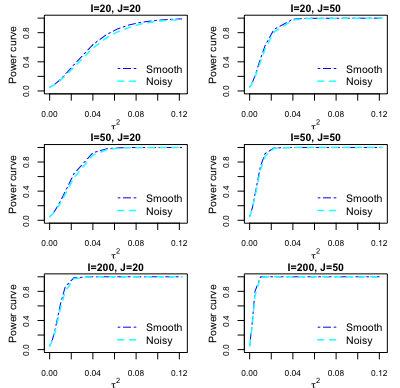
\includegraphics[width=0.9\textwidth]{powercurve.png}
\caption{Power of test ($\tau_k^2=\tau^2$)at the $5\%$ significance level under different model conditions.}
\label{functional power curve}
\end{figure}
In Figure $\ref{functional power curve}$ power curves using both true and noisy $\hat{M}_{I\times J}$ across full combinations of subject number $I$ and visits $J$ are shown. As subject number and visit increase, power of test will be correspondingly increased, and is able to converge to 1 eventually. Under each model condition, test of using true $\hat{M}_{I\times J}$ is more powerful than measurement error considered, i.e. noise added $\hat{M}_{I\times J}$.
\newpage
\subsection{Size Testing To Be Added}
In this section, to compare with our testing procedure, we use the pdIdent model fitting structure in lme approach to fit model under the homoscedasticity assumption, and we would like to show that the size test is too conservative using this method. 

Another method is to fit model under the heteroscedasticity assumption, and then perform multiple test using Bonferroni or benjamini $\&$ Hochberg method.  And we would like to show 
hat the size test is also too conservative using this method. 

\subsection{Power Testing To Be Added}
In the preceding simulation settings, we have shown that our testing procedure by assuming $\tau_k^2=\tau^2$ for all $k$ has good power property when the data is generated following  $\tau_k^2=\tau^2$. In this section, we use heteroscedastic variances $\tau_k^2$ over $k \in \{1,\dots, K\}$ to construct the datasets. Specifically, let $\tau_k^2=\frac{1}{2^{k-1}}\tau^2, k=1,\dots, 3$, and different nonzero $\tau_k^2$s  under the alternative hypothesis are used to generate power curves. 

\begin{figure}[h!]
\centering
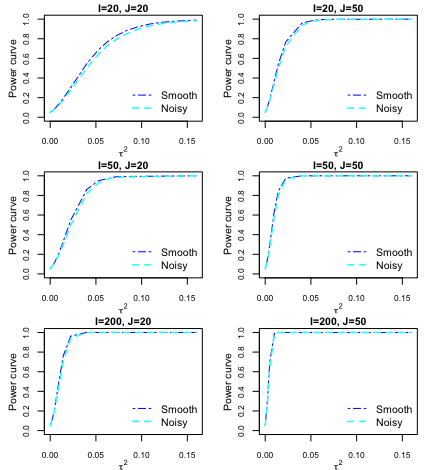
\includegraphics[width=0.9\textwidth]{heter_power_curve.png}
\caption{Power of test ($\tau_k^2=\frac{1}{2^{k-1}}\tau^2$) at the $5\%$ significance level under different model conditions.}
\label{heter functional power curve}
\end{figure}

Figure $\ref{heter functional power curve}$ illustrates the behavior of power when $\tau_k^2$ increases. It shows the similar pattens with data is generated by assuming $\tau_k^2=\tau^2$ for $k \in {1,\dots,3}$ under each of the conditions. That is, power of test will be increased as subject number and visit increase, and power of test will converge to 1. Under each model condition, test of using true $\hat{M}_{I\times J}$ is more powerful than using measurement error added $\hat{M}_{I\times J}$. While under heterogeneous variance, it takes longer for the test of power to increase to 1 compared with using homogeneous variance to construct dataset. 

\subsection{Estimation To Be Added}
Here, in order to evaluate subject-specific derivation $\beta_i(t)$ from the population effect $\beta(t)$ under heteroscedastic variance model, and compare the estimates for population effect $\beta(t)$ from heteroscedastic variance model and no functional random effect model, we consider multiple model conditions.

We generate the response $Y_{ij}$
from model \eqref{eq:lme:approx} with $K=3$, $\delta = 0.5$,
 $\gamma = 2$,
 $\gamma_i \overset{i.i.d.}{\sim} \N(0, 1)$,
 $Z_{ij} \overset{i.i.d.}{\sim} \text{Bernoulli}(0.5)$,
  $\xi_{ijk} \overset{i.i.d.}{\sim} \N(0,\lambda_k)$,
  $\theta = 2$, $\theta_{ik} \overset{i.i.d.}{\sim} \N(0, \tau_i^2)$, $i=1,\dots, K$,
  and  $\epsilon_{ij} \overset{i.i.d.}{\sim} \N(0, 1)$.
  Here, $\lambda_k=0.5^k, k=1,\dots, K$.
 Then the noisy functional data is generated from model \eqref{eq:W}
with $X_{ij}(t) = \sum_{k=1}^K \xi_{ijk} \phi_k(t)$ 
and $e_{ijk}\overset{i.i.d.}{\sim}\N(0,\sigma_W^2)$.
Here, $\phi_1 (t)=\sqrt{2}\mathrm{sin}(2\pi t)$, $\phi_2 (t)=\sqrt{2}\mathrm{cos}(4\pi t)$,$\phi_3 (t)=\sqrt{2}\mathrm{sin}(4\pi t)$, and $\sigma_W^2$ is chosen so 
that the signal to noise ratio in the functional data $r = \sigma_W^{-2}\int_{\tau} r(t,t) \mathrm{d}t$
equals either 0 or 3. Note that $r=0$ corresponds to smooth functional data without noises and 
$r=3$ corresponds to noisy functional data. Finally homogeneous $\tau_i^2$ and heteroscedastic $\tau_i^2$ are considered for variance of interest, to be specific, we take $\tau_1^2=\cdots=\tau_K^2=\tau^2, \tau^2 \in \{0.02, 0.04, 0.08\}$, and $\tau_i^2=\frac{1}{2^{i-1}}\tau^2, i=1,\dots, K, \tau^2 \in \{0.02, 0.04, 0.08\}$ separately. 

A full combination of the number of subject $I$, the number of visits per subject, $J$, the signal to noise ratio $r$ and variance of interest $\tau_i^2 (i=1,\dots,K)$ in the functional data are taken into model conditions consideration. Hence, datasets are constructed under a total of 72 different model conditions: $\big\{(I,J, r, (\tau_i^2, i=1,\dots,K), \tau^2): I\in \{ 20,50,200\}, J\in \{20,50\}, r\in \{0,3\} , (\tau_k^2,  k=1,\dots,K) \in \{ (\tau_1^2=\cdots=\tau_K^2=\tau^2), (\tau_k^2=\frac{1}{2^{k-1}}\tau^2, k=1,\dots, K) \} , \tau^2 \in \{0.02, 0.04, 0.08\} \big\}$.
Under each model condition, 20000 datasets are simulated.

ISE= $\int(\beta(t)-\hat{\beta}(t))^2 \mbox{dt}$ is used to compare estimate performance for population functional effect $\beta(t)$ from heteroscedastic variance model and no functional random effect model. IMSE = $\frac{1}{I} \sum_{i=1}^{I} \int(\beta_i(t)-\hat{\beta}_i(t))^2 \mbox{dt}$ is used for evaluating the subject-specific functional random effect $\beta_i(t)$ estimated by heteroscedastic variance model. Note that ${\beta}(t) = \sum_{k=1}^{K} {\theta}{\phi}_k(t)$, ${\beta}_i(t) = \sum_{k=1}^{K} {\theta}_{ik}{\phi}_k(t), \hat{\beta}(t) = \sum_{k=1}^{K} \hat{\theta}_k\hat{\phi}_k(t)$
and $\hat{\beta}_i(t) = \sum_{k=1}^{K} \hat{\theta}_{ik}\hat{\phi}_k(t)$. MSE=$\frac{1}{I} \sum_{i=1}^{I}\frac{1}{J_i} \sum_{j=1}^{J_i}(y_{ij}-\hat{y}_{ij})^2$ is used to compare predictions from heteroscedastic variance model and no functional random effect model.


